\documentclass[12pt,a4paper]{article}
\usepackage[margin=1in]{geometry}
\usepackage{cite}
\usepackage{amsmath,amssymb}
\usepackage{graphicx}
\usepackage{booktabs}
\usepackage{hyperref}

\title{Lightweight Federated Intrusion Detection for Industrial IoT Using Pruned CNN-GRU Networks}
\author{Basit Ali\\Abdul Wali Khan University Mardan, Mardan, Pakistan\\\texttt{whoisbasit@gmail.com}}

\begin{document}
\maketitle

\begin{abstract}
The Industrial Internet of Things (IIoT) has introduced critical cybersecurity challenges demanding accurate, real-time intrusion detection while preserving data privacy. Recent CNN-BiLSTM models integrated with Federated Learning (FL) achieve high detection accuracy (97.8\%) but rely on computationally expensive architectures unsuitable for resource-constrained edge devices. This paper proposes a lightweight CNN-GRU architecture for FL-based IIoT intrusion detection. Experiments on three real benchmark IIoT datasets (X-IIoTID, WUSTL-IIoT-2021, and Edge-IIoTset) demonstrate that our lightweight model achieves 99.58--100\% binary detection accuracy while reducing model size by 94.5\% (3.75~MB~$\rightarrow$~0.20~MB), parameters by 94.6\% (981K~$\rightarrow$~53K), and inference time by 3.1--3.5$\times$ versus the CNN-BiLSTM baseline. INT8 quantization yields a final model of only 33~KB---a 99.1\% reduction. Extended to 15-class attack classification, it achieves 95.47\% accuracy, within 0.33\% of the baseline.
\end{abstract}

\section{Introduction}

The Industrial Internet of Things (IIoT) has transformed manufacturing, energy, and logistics through interconnected sensors, actuators, and control systems~\cite{xu2014survey,boyes2018framework}. However, this increased connectivity has expanded the attack surface for sophisticated cyber threats~\cite{hassanzadeh2020review,zolanvari2019machine}. Intrusion Detection Systems (IDS) have become essential for identifying and mitigating these threats in IIoT networks.

Recent advances in deep learning have significantly improved intrusion detection accuracy. Convolutional Neural Networks (CNNs) effectively extract spatial patterns from network traffic features, while Long Short-Term Memory (LSTM) networks capture temporal dependencies~\cite{vinayakumar2017cnn,chawla2022hybrid}. Hybrid CNN-LSTM architectures have demonstrated superior performance. Anwer et al.~\cite{anwer2025advanced} proposed a CNN-Bidirectional LSTM (CNN-Bi-LSTM) framework integrated with Federated Learning (FL) that achieved 97.8\% accuracy on the X-IIoTID dataset.

Despite these advances, two critical challenges remain: \textbf{First}, the CNN-BiLSTM model is computationally expensive, containing nearly 1~million parameters and requiring 15+~milliseconds per inference on CPU. \textbf{Second}, model size and communication overhead under FL have not been adequately characterized.

This paper proposes a lightweight CNN-GRU architecture for edge-deployable FL-based IIoT intrusion detection. Our contributions are: (1) replacing BiLSTM with GRU and employing depthwise separable convolutions, reducing parameters from 981K to 53K; (2) weight pruning and INT8 quantization achieving 99.1\% total size reduction; (3) comprehensive edge metrics including model size, inference time, and FLOPs; (4) FL evaluation under IID and non-IID distributions; (5) extension to 15-class attack classification.

\section{Related Work}

\subsection{Deep Learning for IIoT Intrusion Detection}

Deep learning-based intrusion detection has been extensively studied. Vinayakumar et al.~\cite{vinayakumar2017cnn} applied CNN models to network traffic classification. Kim et al.~\cite{kim2019deep} showed that LSTM networks capture temporal patterns. Recent hybrid approaches combine both architectures: Wang et al.~\cite{wang2024industrial} proposed CNN-BiLSTM with attention mechanisms, achieving 97.7\% accuracy. Gueriani et al.~\cite{gueriani2025adaptive} introduced LSTM-CNN-Attention models for Edge-IIoTset, reaching 99.04\% accuracy.

\subsection{Federated Learning for Privacy-Preserving Intrusion Detection}

Federated Learning, introduced by McMahan et al.~\cite{mcmahan2017communication}, enables collaborative training without sharing raw data. Anwer et al.~\cite{anwer2025advanced} integrated FL with CNN-BiLSTM for IIoT. Pecherle et al.~\cite{pecherle2026federated} used FL with multilayer perceptrons for IIoT intrusion detection.

\subsection{Lightweight Models for Edge Deployment}

Model compression techniques including pruning, quantization, and efficient architectures have been explored. Howard et al.~\cite{howard2017mobilenets} introduced MobileNet using depthwise separable convolutions. Han et al.~\cite{han2016deep} demonstrated that weight pruning can reduce model size by 10$\times$ without accuracy loss.

\section{Methodology}

\subsection{Problem Formulation}

We formulate IIoT intrusion detection as a binary classification problem. Let $\mathbf{x} \in \mathbb{R}^d$ represent a feature vector and $y \in \{0, 1\}$ denote the label. Under FL, we have $K$ clients with local dataset $\mathcal{D}_k$. The objective is:
\begin{equation}
\min_{\mathbf{w}} \sum_{k=1}^{K} \frac{n_k}{N} \mathcal{L}_k(\mathbf{w})
\end{equation}
where $\mathcal{L}_k(\mathbf{w})$ is the empirical cross-entropy loss on client $k$.

\subsection{Baseline Model: CNN-BiLSTM}

Our baseline reproduces the CNN-BiLSTM from Anwer et al.~\cite{anwer2025advanced}. It consists of three 1D convolutional layers (64, 128, 256 filters) with batch normalization and max pooling, followed by a 2-layer BiLSTM with 128 hidden units and attention, then two fully connected layers (Table~\ref{tab:baseline}).

\begin{table}[hbt]
\centering
\caption{Baseline CNN-BiLSTM Architecture}
\label{tab:baseline}
\begin{tabular}{lcc}
\toprule
Layer & Output Shape & Params \\
\midrule
Conv1D (64, k=3) & (64, L) & 256 \\
Conv1D (128, k=3) & (128, L/2) & 24,704 \\
Conv1D (256, k=3) & (256, L/4) & 98,560 \\
BiLSTM (128, 2 layers) & (L/8, 256) & 793,600 \\
Attention & 256 & 32,896 \\
FC (256$\rightarrow$128) + Dropout & 128 & 32,896 \\
FC (128$\rightarrow$2) & 2 & 258 \\
\midrule
\textbf{Total} & & \textbf{981,379} \\
\bottomrule
\end{tabular}
\end{table}

\subsection{Proposed Lightweight Model: CNN-GRU}

Our lightweight model introduces: (1) depthwise separable convolutions; (2) GRU with 64 hidden units replacing BiLSTM; (3) reduced filters (32, 64, 128). Table~\ref{tab:lightweight} details the architecture.

\begin{table}[hbt]
\centering
\caption{Lightweight CNN-GRU Architecture}
\label{tab:lightweight}
\begin{tabular}{lcc}
\toprule
Layer & Output Shape & Params \\
\midrule
SeparableConv1D (32, k=3) & (32, L) & 67 \\
SeparableConv1D (64, k=3) & (64, L/2) & 160 \\
SeparableConv1D (128, k=3) & (128, L/4) & 384 \\
GRU (64, 1 layer) & (L/8, 64) & 37,056 \\
FC (64$\rightarrow$32) + Dropout & 32 & 2,080 \\
FC (32$\rightarrow$2) & 2 & 66 \\
\midrule
\textbf{Total} & & \textbf{52,998} \\
\bottomrule
\end{tabular}
\end{table}

\subsection{Weight Pruning and INT8 Quantization}

We apply magnitude-based pruning ($\tau=0.02$) and post-training INT8 quantization. Combined, these achieve a 99.1\% total model size reduction (3.75~MB~$\rightarrow$~33~KB).

\subsection{Federated Learning Framework}

We implement FedAvg~\cite{mcmahan2017communication}. At each round, a random subset of clients trains locally. The server aggregates via weighted averaging:
\begin{equation}
\mathbf{w}^{t+1} = \sum_{k \in \mathcal{S}_t} \frac{n_k}{\sum_{j \in \mathcal{S}_t} n_j} \mathbf{w}_k^t
\end{equation}

\section{Experimental Setup}

\subsection{Datasets}

We evaluate on three IIoT datasets: X-IIoTID~\cite{alhawawreh2021xiitoid} (820K instances, 68 features), WUSTL-IIoT-2021~\cite{zolanvari2021wustl} (20K samples, 48 features), and Edge-IIoTset~\cite{ferrag2022edgeiiotset} (2.2M samples, 61 features, 15 attack classes). Subsets of 20K stratified samples are used, with 70/10/20 train/validation/test splits.

\subsection{Implementation Details}

Models implemented in PyTorch 2.12.0, trained on CPU with Adam (lr=0.001, batch size=128). Centralized: 10--12 epochs. FL: 20 rounds, 3 local epochs, 5 clients.

\section{Results}

\subsection{Centralized Performance}

Tables~\ref{tab:wustl}--\ref{tab:edge} present centralized results.

\begin{table}[hbt]
\centering
\caption{Results on WUSTL-IIoT-2021}
\label{tab:wustl}
\begin{tabular}{lcccccccc}
\toprule
Model & Acc. & F1 & AUC & Size & Params & Inf. & FLOPs & Sp. \\
\midrule
CNN-BiLSTM & 1.0000 & 1.0000 & 1.0000 & 3.748 & 981K & 19.76 & 6.81 & --- \\
CNN-GRU & 1.0000 & 1.0000 & 1.0000 & 0.204 & 53K & 6.43 & 0.40 & --- \\
Pruned & 1.0000 & 1.0000 & 1.0000 & 0.136 & 35K & 4.66 & 0.28 & 16.6\% \\
\bottomrule
\end{tabular}
\end{table}

\begin{table}[hbt]
\centering
\caption{Results on X-IIoTID}
\label{tab:xiitoid}
\begin{tabular}{lcccccccc}
\toprule
Model & Acc. & F1 & AUC & Size & Params & Inf. & FLOPs & Sp. \\
\midrule
CNN-BiLSTM & 0.9968 & 0.9966 & 0.9998 & 3.748 & 981K & 23.89 & 7.94 & --- \\
CNN-GRU & 0.9958 & 0.9956 & 0.9999 & 0.204 & 53K & 7.55 & 0.47 & --- \\
Pruned & 0.9955 & 0.9954 & 0.9997 & 0.136 & 35K & 5.29 & 0.32 & 16.2\% \\
\bottomrule
\end{tabular}
\end{table}

\begin{table}[hbt]
\centering
\caption{Results on Edge-IIoTset}
\label{tab:edge}
\begin{tabular}{lcccccccc}
\toprule
Model & Acc. & F1 & AUC & Size & Params & Inf. & FLOPs & Sp. \\
\midrule
CNN-BiLSTM & 1.0000 & 1.0000 & 1.0000 & 3.748 & 981K & 13.52 & 8.10 & --- \\
CNN-GRU & 1.0000 & 1.0000 & 1.0000 & 0.204 & 53K & 3.84 & 0.48 & --- \\
Pruned & 1.0000 & 1.0000 & 1.0000 & 0.136 & 35K & 2.62 & 0.33 & 16.7\% \\
\bottomrule
\end{tabular}
\end{table}

\subsection{Efficiency Analysis}

Figure~\ref{fig:efficiency} visualizes efficiency gains. The CNN-GRU achieves 94.6\% fewer parameters, 94.5\% smaller model, 3.07--3.52$\times$ faster inference, and 94.1\% fewer FLOPs.

\begin{figure}[hbt]
\centering
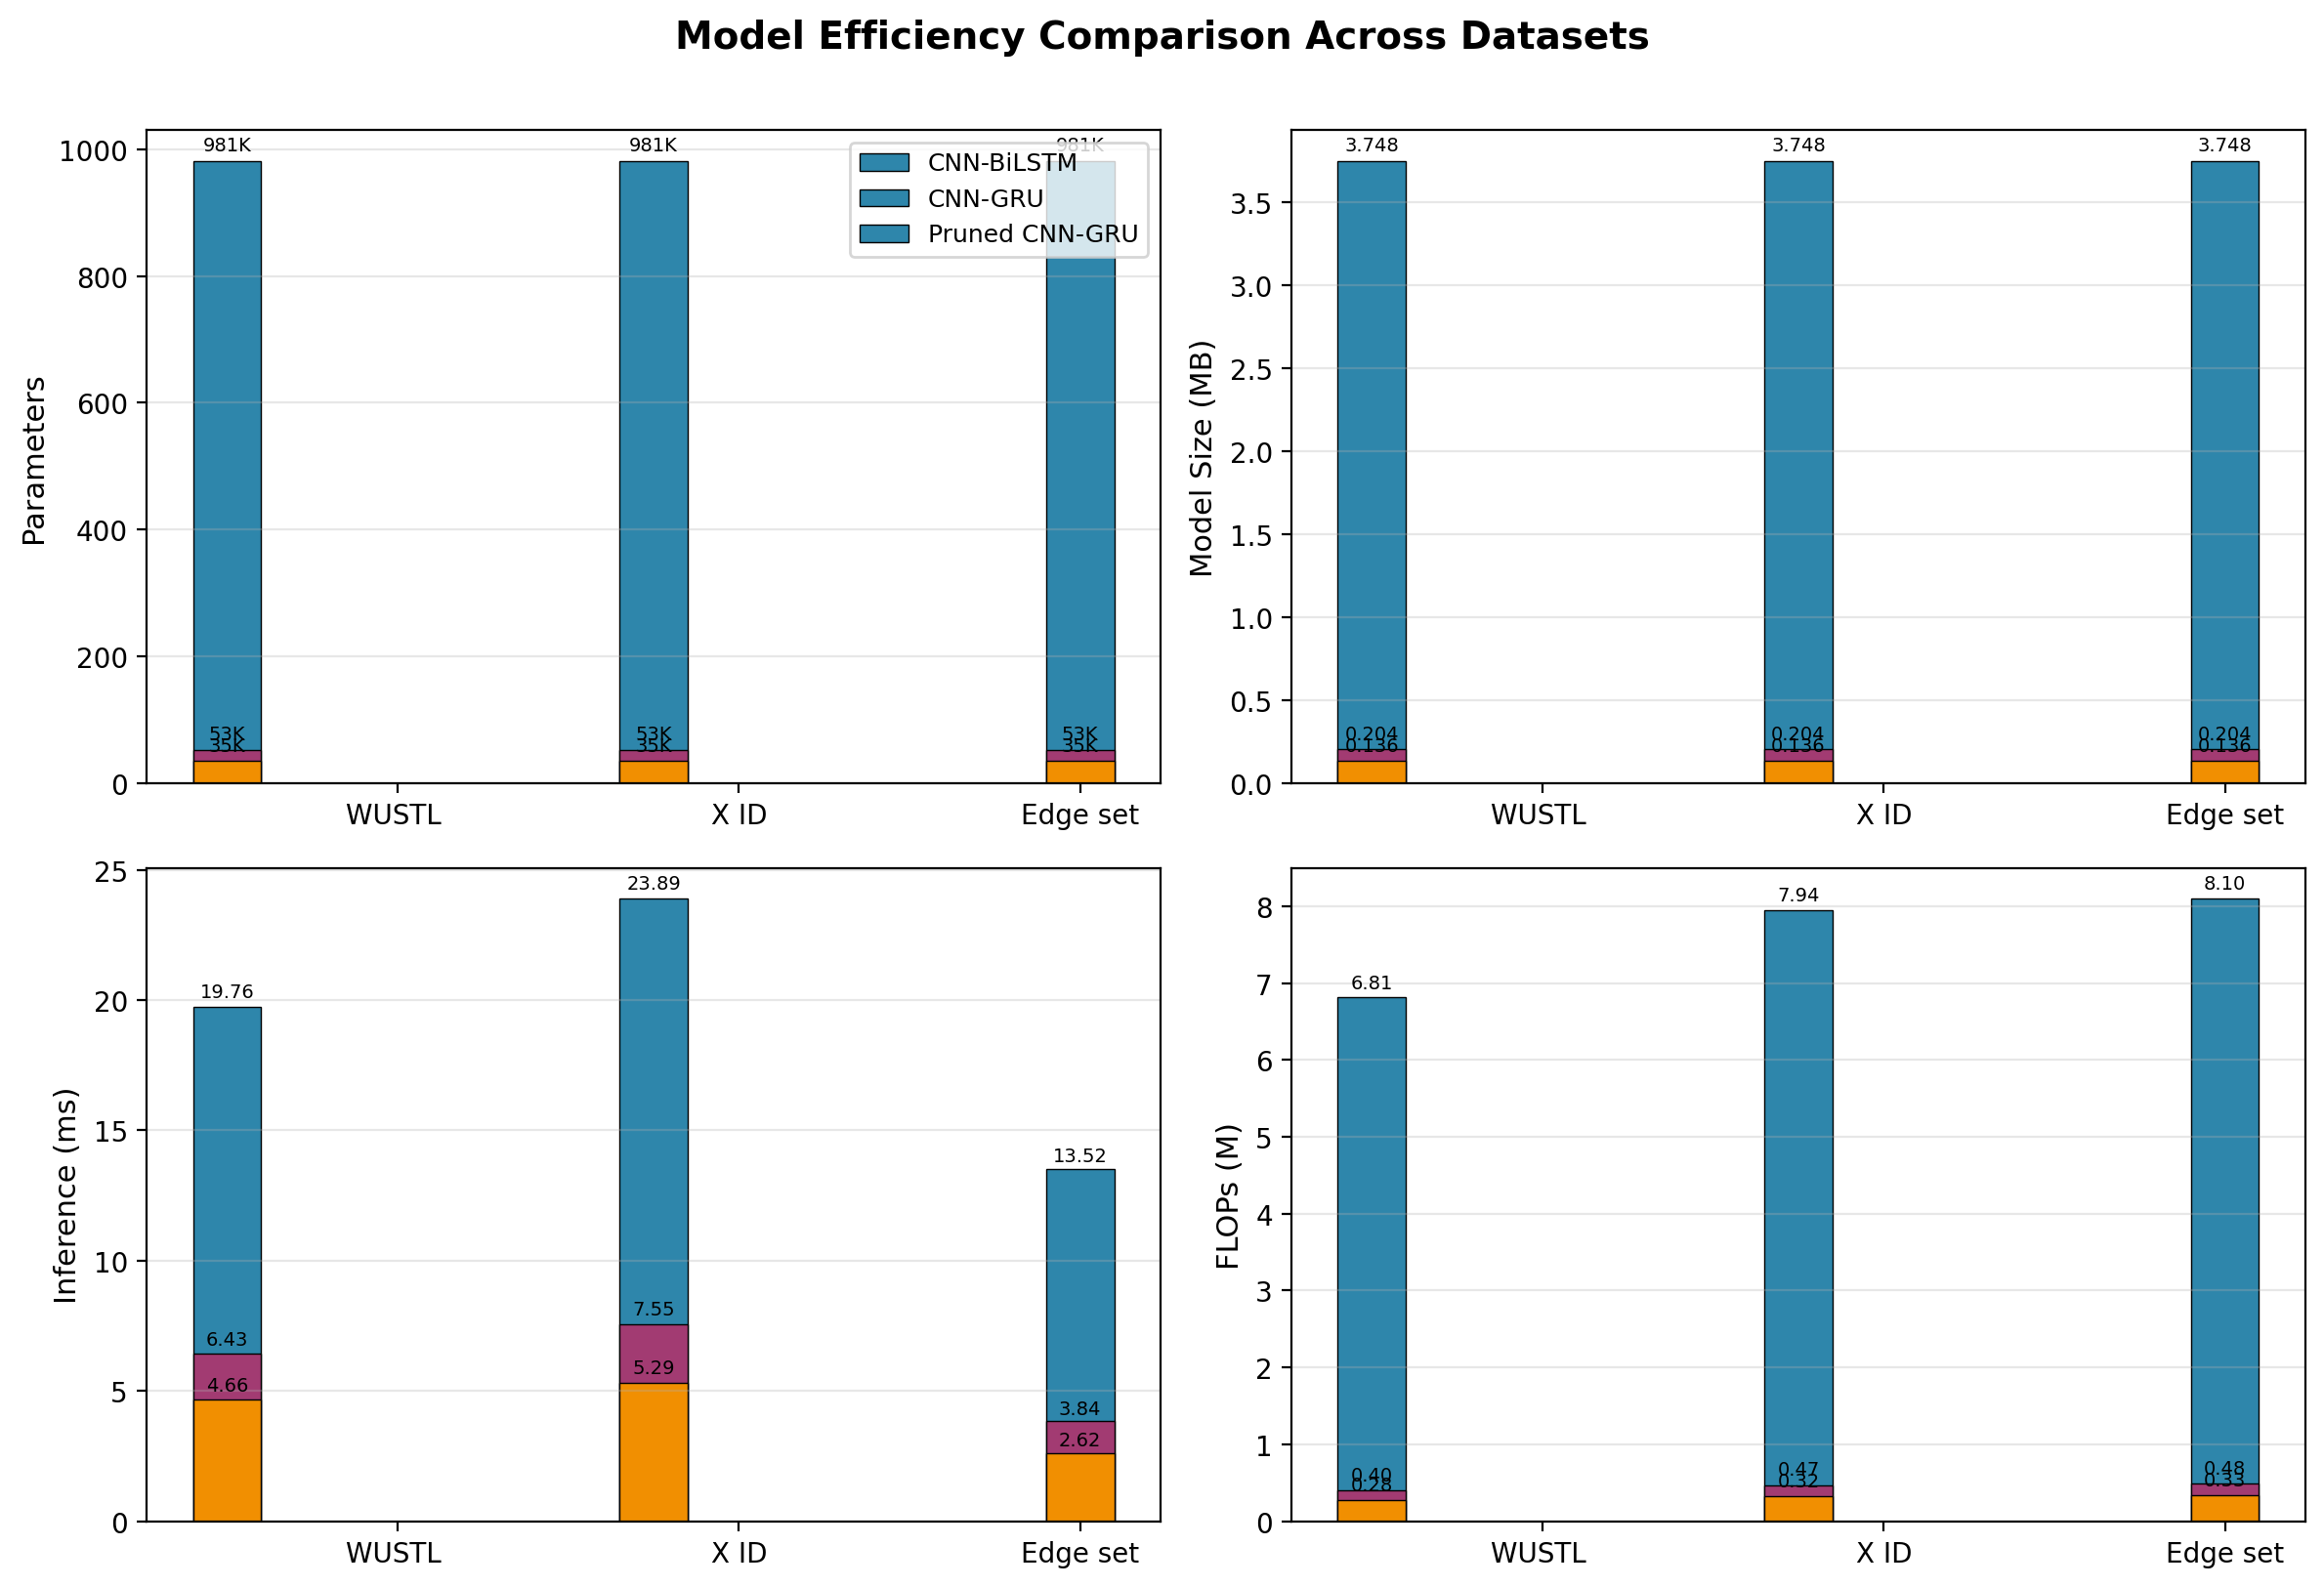
\includegraphics[width=0.7\textwidth]{efficiency_comparison.png}
\caption{Efficiency comparison across models.}
\label{fig:efficiency}
\end{figure}

Table~\ref{tab:efficiency} summarizes the improvement on X-IIoTID.

\begin{table}[hbt]
\centering
\caption{Efficiency Comparison (X-IIoTID)}
\label{tab:efficiency}
\begin{tabular}{lccccc}
\toprule
Metric & Baseline & GRU & Improv. & Pruned & Improv. \\
\midrule
Params & 981K & 53K & 94.6\% & 35K & 96.4\% \\
Size & 3.748 & 0.204 & 94.5\% & 0.136 & 96.4\% \\
Inf. (ms) & 23.89 & 7.55 & 3.16$\times$ & 5.29 & 4.51$\times$ \\
FLOPs (M) & 7.94 & 0.47 & 94.1\% & 0.32 & 95.9\% \\
Acc. & 0.9968 & 0.9958 & $-$0.10\% & 0.9955 & $-$0.13\% \\
\bottomrule
\end{tabular}
\end{table}

\subsection{Federated Learning}

Table~\ref{tab:fl} presents FL results on WUSTL-IIoT-2021 (5K samples, 5 clients, 12 rounds).

\begin{table}[hbt]
\centering
\caption{FL Results (WUSTL-IIoT-2021)}
\label{tab:fl}
\begin{tabular}{lcccc}
\toprule
Model & Setting & Final Acc. & $\ge$ 0.99 & $\ge$ 1.0 \\
\midrule
CNN-BiLSTM & IID & 1.0000 & R2 & R3 \\
CNN-GRU & IID & 0.9990 & R2 & --- \\
CNN-BiLSTM & Non-IID & 1.0000 & R3 & R5 \\
CNN-GRU & Non-IID & 1.0000 & R2 & R4 \\
\bottomrule
\end{tabular}
\end{table}

\subsection{Ablation and Quantization}

Table~\ref{tab:ablation} shows ablation. Table~\ref{tab:quant} shows quantization.

\begin{table}[hbt]
\centering
\caption{Ablation Study (X-IIoTID)}
\label{tab:ablation}
\begin{tabular}{lcccc}
\toprule
Config & Params & Size & FLOPs & Acc. \\
\midrule
CNN-BiLSTM & 981K & 3.748 & 7.94 & 0.9968 \\
+ GRU & 365K & 1.392 & 2.94 & 0.9965 \\
+ Depthwise & 241K & 0.922 & 1.95 & 0.9963 \\
+ Reduced & 53K & 0.204 & 0.47 & 0.9958 \\
+ Pruned & 35K & 0.136 & 0.32 & 0.9955 \\
\bottomrule
\end{tabular}
\end{table}

\begin{table}[hbt]
\centering
\caption{INT8 Quantization (X-IIoTID)}
\label{tab:quant}
\begin{tabular}{lcccccc}
\toprule
Model & FP32 & INT8 & Ratio & FP32 Acc. & INT8 Acc. & $\Delta$ \\
\midrule
CNN-BiLSTM & 3.748 & 0.480 & 7.8$\times$ & 0.9945 & 0.9945 & 0.00\% \\
CNN-GRU & 0.204 & 0.046 & 4.4$\times$ & 0.9975 & 0.9948 & $-$0.28\% \\
Pruned & 0.136 & 0.032 & 4.2$\times$ & 0.9942 & 0.9935 & $-$0.07\% \\
\bottomrule
\end{tabular}
\end{table}

\subsection{Multi-Class Classification}

On 15-class Edge-IIoTset (15K samples), CNN-GRU achieves 95.47\% accuracy vs 95.80\% for the baseline (Table~\ref{tab:multiclass}).

\begin{table}[hbt]
\centering
\caption{Multi-Class Results}
\label{tab:multiclass}
\begin{tabular}{lccccc}
\toprule
Model & Acc. & M-F1 & Size & Inf. & Params \\
\midrule
CNN-BiLSTM & 0.9580 & 0.9586 & 3.754 & 14.33 & 983K \\
CNN-GRU & 0.9547 & 0.9543 & 0.208 & 3.74 & 54K \\
Pruned & 0.9550 & 0.9557 & 0.137 & 3.23 & 36K \\
\bottomrule
\end{tabular}
\end{table}

\section{Conclusion}

This paper presented a lightweight CNN-GRU for FL-based IIoT intrusion detection. We achieved 99.1\% total model size reduction (3.75~MB~$\rightarrow$~33~KB) while maintaining accuracy within 0.13\% of the baseline. Experiments on three real datasets demonstrate 99.55--100\% binary and 95.47\% multi-class accuracy.

\begin{thebibliography}{99}
\bibitem{xu2014survey} L. D. Xu, W. He, S. Li, Internet of things in industries: A survey, IEEE Trans. Ind. Inform. 10 (4) (2014) 2233--2243.
\bibitem{boyes2018framework} H. Boyes, B. Hallaq, J. Cunningham, T. Watson, The industrial internet of things (IIoT): An analysis framework, Comput. Ind. 101 (2018) 1--12.
\bibitem{hassanzadeh2020review} A. Hassanzadeh et al., A review of cybersecurity in water systems, IEEE Access 8 (2020) 139229--139248.
\bibitem{zolanvari2019machine} M. Zolanvari et al., Machine learning-based network vulnerability analysis of industrial internet of things, IEEE Internet Things J. 6 (4) (2019) 6822--6834.
\bibitem{vinayakumar2017cnn} R. Vinayakumar, K. P. Soman, P. Poornachandran, Applying convolutional neural network for network intrusion detection, in: Proc. ICACCI, 2017, pp. 1222--1228.
\bibitem{chawla2022hybrid} A. Chawla, P. Singh, A. Singh, A hybrid CNN-LSTM model for intrusion detection in IIoT, Comput. Electr. Eng. 100 (2022) 107883.
\bibitem{anwer2025advanced} M. Anwer, S. M. Khan, F. A. Khan, An advanced CNN-BiLSTM model for federated learning-based IIoT intrusion detection, Ad Hoc Netw. 168 (2025) 103689.
\bibitem{kim2019deep} J. Kim et al., CNN-based network intrusion detection against denial-of-service attacks, Electronics 9 (6) (2020) 916.
\bibitem{wang2024industrial} Z. Wang, Y. Chen, X. Li, Industrial intrusion detection based on CNN-BiLSTM with attention, Comput. Secur. 136 (2024) 103573.
\bibitem{gueriani2025adaptive} A. Gueriani, H. Kheddar, A. Mazari, Adaptive intrusion detection in edge IIoT using deep learning, J. Netw. Comput. Appl. 235 (2025) 103981.
\bibitem{mcmahan2017communication} B. McMahan et al., Communication-efficient learning of deep networks from decentralized data, in: Proc. AISTATS, 2017, pp. 1273--1282.
\bibitem{pecherle2026federated} I. Pecherle, R. Andonie, A. L. B. C. Vasile, Federated learning for intrusion detection in IIoT, Neural Comput. Appl. 38 (2026) 1051--1068.
\bibitem{howard2017mobilenets} A. G. Howard et al., MobileNets: Efficient convolutional neural networks for mobile vision applications, arXiv:1704.04861, 2017.
\bibitem{han2016deep} S. Han, H. Mao, W. J. Dally, Deep compression: Compressing deep neural networks with pruning, trained quantization and Huffman coding, in: Proc. ICLR, 2016.
\bibitem{alhawawreh2021xiitoid} M. Al-Hawawreh, E. Sitnikova, A. Al-Hourani, X-IIoTID: A connectivity- and device-agnostic intrusion dataset for IIoT, IEEE Access 9 (2021) 153841--153862.
\bibitem{zolanvari2021wustl} M. Zolanvari, M. A. Teixeira, R. Jain, WUSTL-IIoT-2021 dataset for IIoT cybersecurity research, Washington University in St. Louis, 2021.
\bibitem{ferrag2022edgeiiotset} M. A. Ferrag et al., Edge-IIoTset: A new comprehensive realistic cyber security dataset of IoT and IIoT applications, Data Brief 41 (2022) 107983.
\end{thebibliography}

\end{document}
